\section{Architecture}
The platform should be able to accomodate the ability for teachers to create a syllabus that includes sessions, exercises and test cases for the exercises. Additionally, the platform should have the ability for students to do the exercises that the teacher has provided. 

The platform should be a web application, consisting of a user-interface, business logic to handle requests, authentication and compilation of the code as well as a database to persist relevant data.

Based on these requirements we have created the architecture seen in figure \ref{fig:Architecture}.

\begin{figure}[H]
	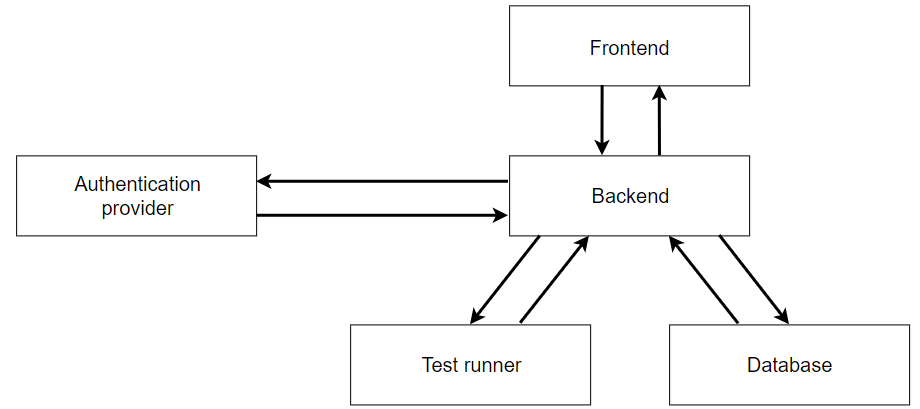
\includegraphics[scale=0.6]{Architecture.PNG}
	\centering
	\caption{The architecture for the web application}
	\label{fig:Architecture}
\end{figure}

In the following sections we will describe the general structure of each component and its responsibility.

\subsubsection{Frontend}
The frontend is the user facing component of our web application. The frontend is designed such that the user-interface and the functionality on the frontend is dependent on the role of the user. 
For example if the signed in user has a student role, the user will be able to see and complete exercises, where if the user has a role of teacher, they will have access to more functionality such as creating a syllabus or exercise.

Therefore the responsibility of the frontend can be split into two categories: 
\begin{itemize}
    \item \textbf{Teacher}-based responsibilities and,
    \item \textbf{Student}-based responsibilities.
\end{itemize}

\subsubsection*{Teacher-based responsibilities}
If the signed in user is a teacher the frontend the frontend provides the user the ability to create syllabi, sessions, exercises and test cases for the given exercise, as well as they ability to complete exercises. The latter functionality was included to allow teachers to try out the exercises and ensure that the test cases behave as expected before releasing the exercise to the students.

\subsubsection*{Student-based responsibilities}

%Describe the following:
%1. The system must be able to provide a suitable UI for the user, but should not use their computer for anything else 
%2. The system must be able to provide some way to execute haskell code and assert whether or not the code is correct. 
%3. .... therefore we choose to split the system into multiple subsystem, each being responsible for providing different functionalities to the full system and can run independently of one another. 
%4. .... by doing this we gain.....

% Why do we choose the front end we do --- why do we have the 'front end backend?' --- Is the front end system only on the client? No? Why not?

\subsection{Back-end system}


\subsubsection{Code runner}
Our system needs to be able to compile and run haskell code on back-end and verify whether this code is syntactically correct or not.
To accomodate this, a code runner module has been implement in a layered architecture (\ref{røde aalborg}).
For this type of architecture each component can depend only on components on a lower or same level, thus if component A is on a lower level than component B, component A cannot use component B.
The component is implemented as a HTTP server as seen on Figure \ref{fig:code_runner}.
Whenever the server recieves a HTTP request, a service request is sent to a \textit{code runner} service that in turn writes the content recieved to a Haskell file and invokes the GHC compiler.
If the compilation of the haskell file fails, the code runner will send the GHC compiler's compilation error as response to the service user.
If the file compiles successfully the code runner will then run the executable file and fetch the produced output of the program.
This output is then sent to the service user.
Finally, the response from the code runner, whether successful or not, is redirected back to the client, providing them with information about the compilation and execution.



\subsection{Front-end system}

\subsubsection{UI}

\subsubsection{UI business layer}